\subsection{tempPerDay()}

The third graph we created was the second example graph proposed in the instructions file. It shows the mean temperature for each day of the year. It is produced by the member function of tempTrender called "tempPerDay(). Conceptually, it is similar to stacking 365 of the "tempOnDay()" histograms vertically. It was created by using the ROOT histogram class "TProfile".
Data parsing was identical to the parsing done for graphs 1 and 2. 

\begin{figure}[h]
\centering
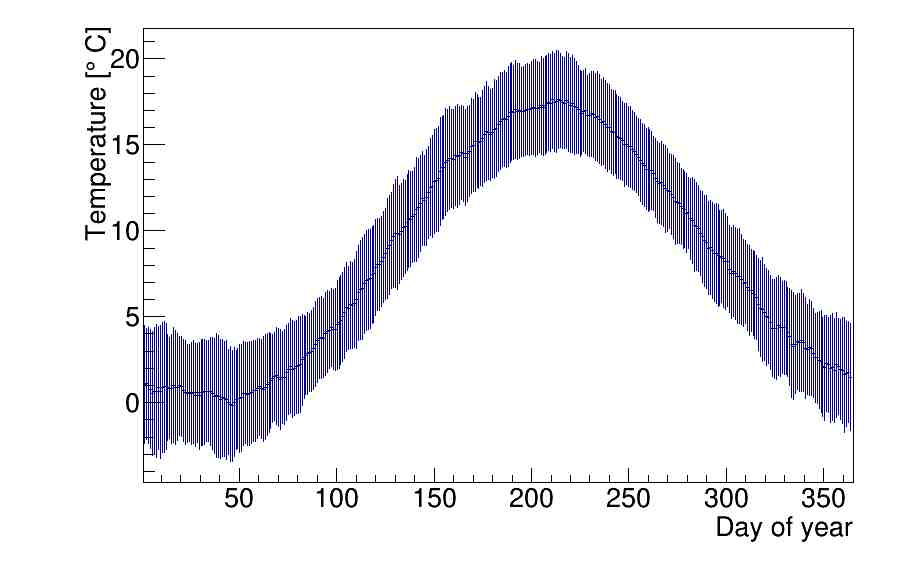
\includegraphics[scale=0.3]{graph3.png}
\caption{Histogram showing the mean temperature on each day of the year. Produced by "tempPerDay()". }
\end{figure}